\newcommand{\institut}{Institut f\"ur Energie und  Automatisiertungstechnik}
\newcommand{\fachgebiet}{Elektronische Mess- und Diagnosetechnik}
\newcommand{\veranstaltung}{Praktikum Messdatenverarbeitung}
\newcommand{\pdfautor}{\"Ozg\"u Dogan (326 048), Timo Lausen (325 411), Boris Henckell (325 779)}
\newcommand{\autor}{\"Ozg\"u Dogan (326 048)\\ Timo Lausen (325 411)\\ Boris Henckell (325 779)}
\newcommand{\pdftitle}{Praktikum Messdatenverarbeitung  Termin 3 und 4}
\newcommand{\prototitle}{Praktikum Messdatenverarbeitung \\ Termin 3 und 4}
\newcommand{\aufgabe}{}

\newcommand{\gruppe}{Gruppe: G1 Fr 08-10}
\newcommand{\betreuer}{Betreuer: J\"urgen Funk}

\input{../../packages/tu_header_8}
%---------------------------------------------------------------------
%---------------------------------------------------------------------
%---------------------------------------------------------------------

\section{Vorbereitungsaufgaben}
\begin{quote}
    \subsection{Sinusfunktion erzeugen und DFT erstellen}
    \begin{quote}
        siehe Quelltext sinus2.m im Anhang
        \begin{figure}[H]
        \centering
            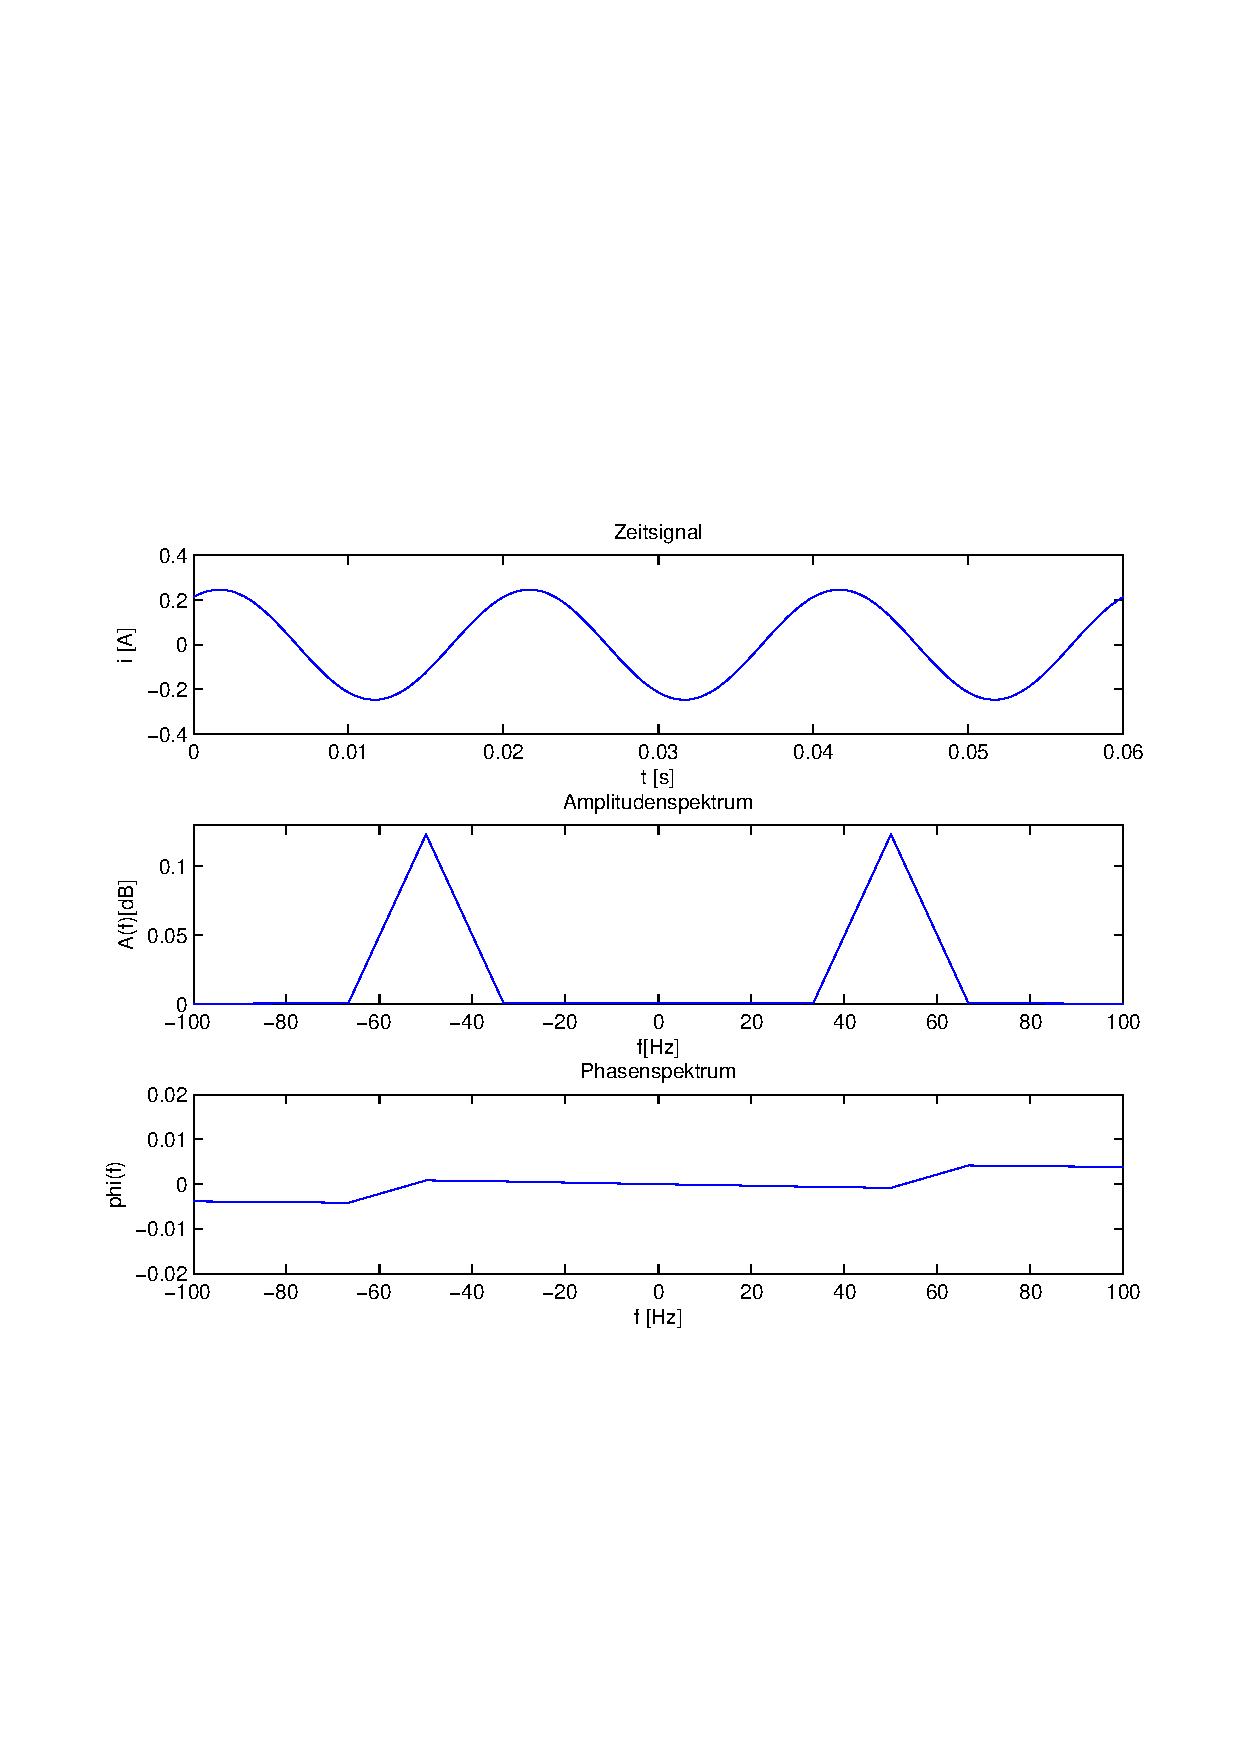
\includegraphics[scale=0.5, trim = 0cm 0cm 0cm 0cm, clip]{./Bilder/VerschobenerSinusAufgabe1}
                \caption{Verschobener Sinus}
                \label{fig:./Bilder/VerschobenerSinusAufgabe1}
        \end{figure}
    
    \end{quote}
    
	\subsection{Angeschnittene Sinusfunktion}
    \begin{quote}
        Siehe Quelltext stromPhasSchnitt.m im Anhang\\
        Um diese Funktion zu erstellen haben wir eine for Schleife imlementiert, die den gesamten zeitvektor t
        durchläuft. Für jeden Durchlauf wird getestet, wo sich der jeweilige Zeitpunkt im Verhältniss zum halben
        sinussignal befindet. Anschließend wird in der if abfrage bestimmt, ob sich dieser Zeitpunkt relativ zur halben
        Periode des Sinussignals vor oder hinter dem Phasenanschnittswinkel befindet. Abhängig davon wird der
        dentsprechenden Stelle im Ausgabevektor der Wert $0$ oder der Wert den die Sinusfunktion ermittelt, übergeben.\\
        Für die Phasenanschnittswinkel. $ \alpha = 0, \frac{1}{8} \pi, \frac{1}{4} \pi, \frac{3}{8} \pi, \frac{1}{2}
        \pi,\frac{5}{8} \pi, \frac{3}{4} \pi, \frac{7}{8} \pi$ und $\pi$ ergeben sich folgende 
    \end{quote}
    
    \subsection{Effektivwert des Stroms im Zeitbereich}
    \begin{quote}
        Siehe Quelltext EffektivwertZeitbereich.m im Anhang\\
        Für den Effektivwert des Stroms im Zeitbereich ermitteln wir die Wurzel des Mittelwertes des Quadrats des
        Stromvektors.
    \end{quote}
    
    \subsection{Effektivwert des Stroms im Frequenzbereich}
    \begin{quote}
        Siehe Quelltext EffektivwertFourier.m im Anhang\\
        Den Effektivwert des Stroms im Frequenzbereich ermitteln wir ähnlich wie den Effektivwert des Stroms im
        Zeitbereich. Dank des Parsevalschen-Theorems \ldots
        \end{quote}
    \subsection{Ergebnisse Vorbereitungsaufgaben}
    \begin{quote}
                                %4 Grafiken:
            \begin{center}
            \begin{tabular}{ll}

            \hspace{-11em}
                \begin{minipage}{0.6\textwidth}

                    \begin{figure}[H]
                        \label{fig:}
                        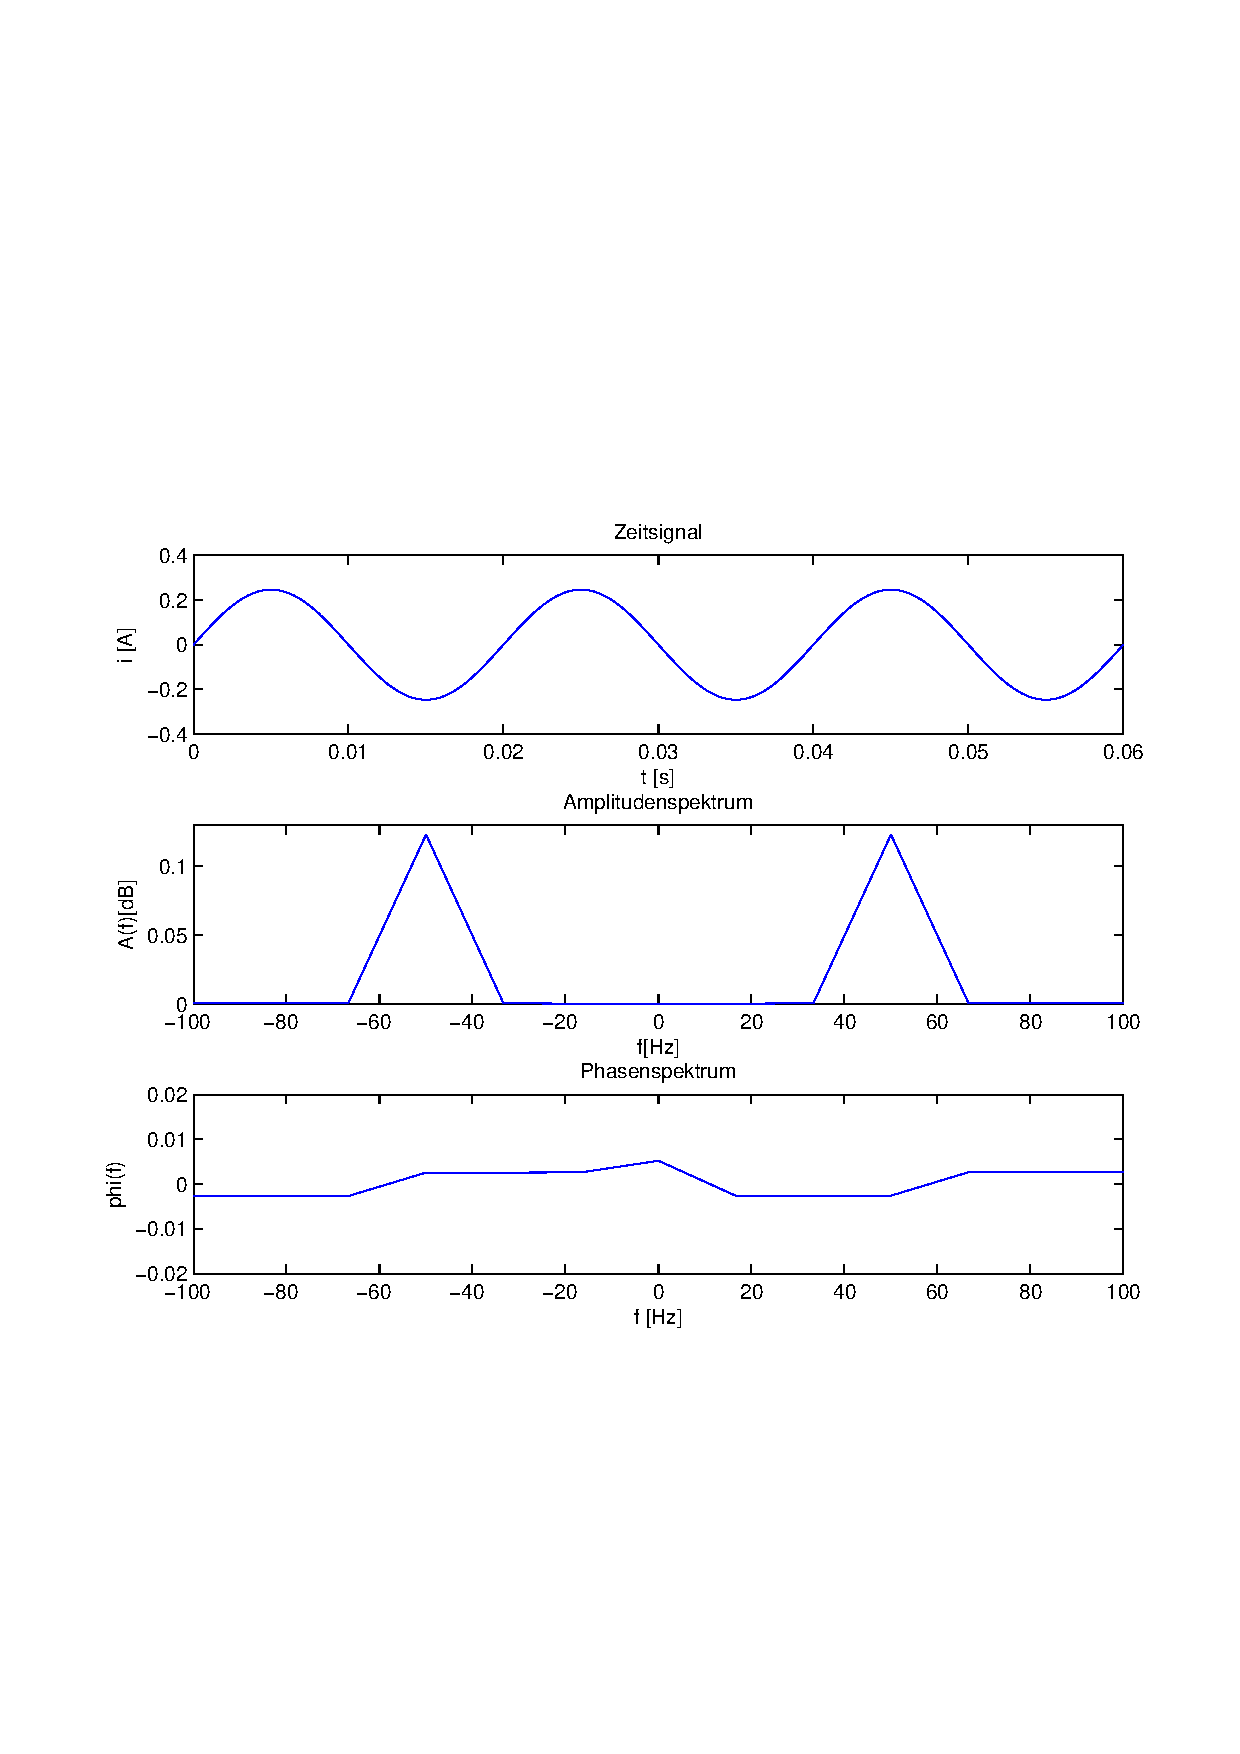
\includegraphics[scale=0.5, trim = 2cm 7cm 1.5cm 8.5cm, clip]{./Bilder/Phasenanschnitt08pi.pdf}
                        %FIXME [width=640px,
                         %height=474px]
                        \caption{Sinussignal mit Phasenanschnitt von $0$}
                    \end{figure}

                \end{minipage}
                \begin{minipage}{0.6\textwidth}

                    \begin{figure}[H]
                        \label{fig:}
                        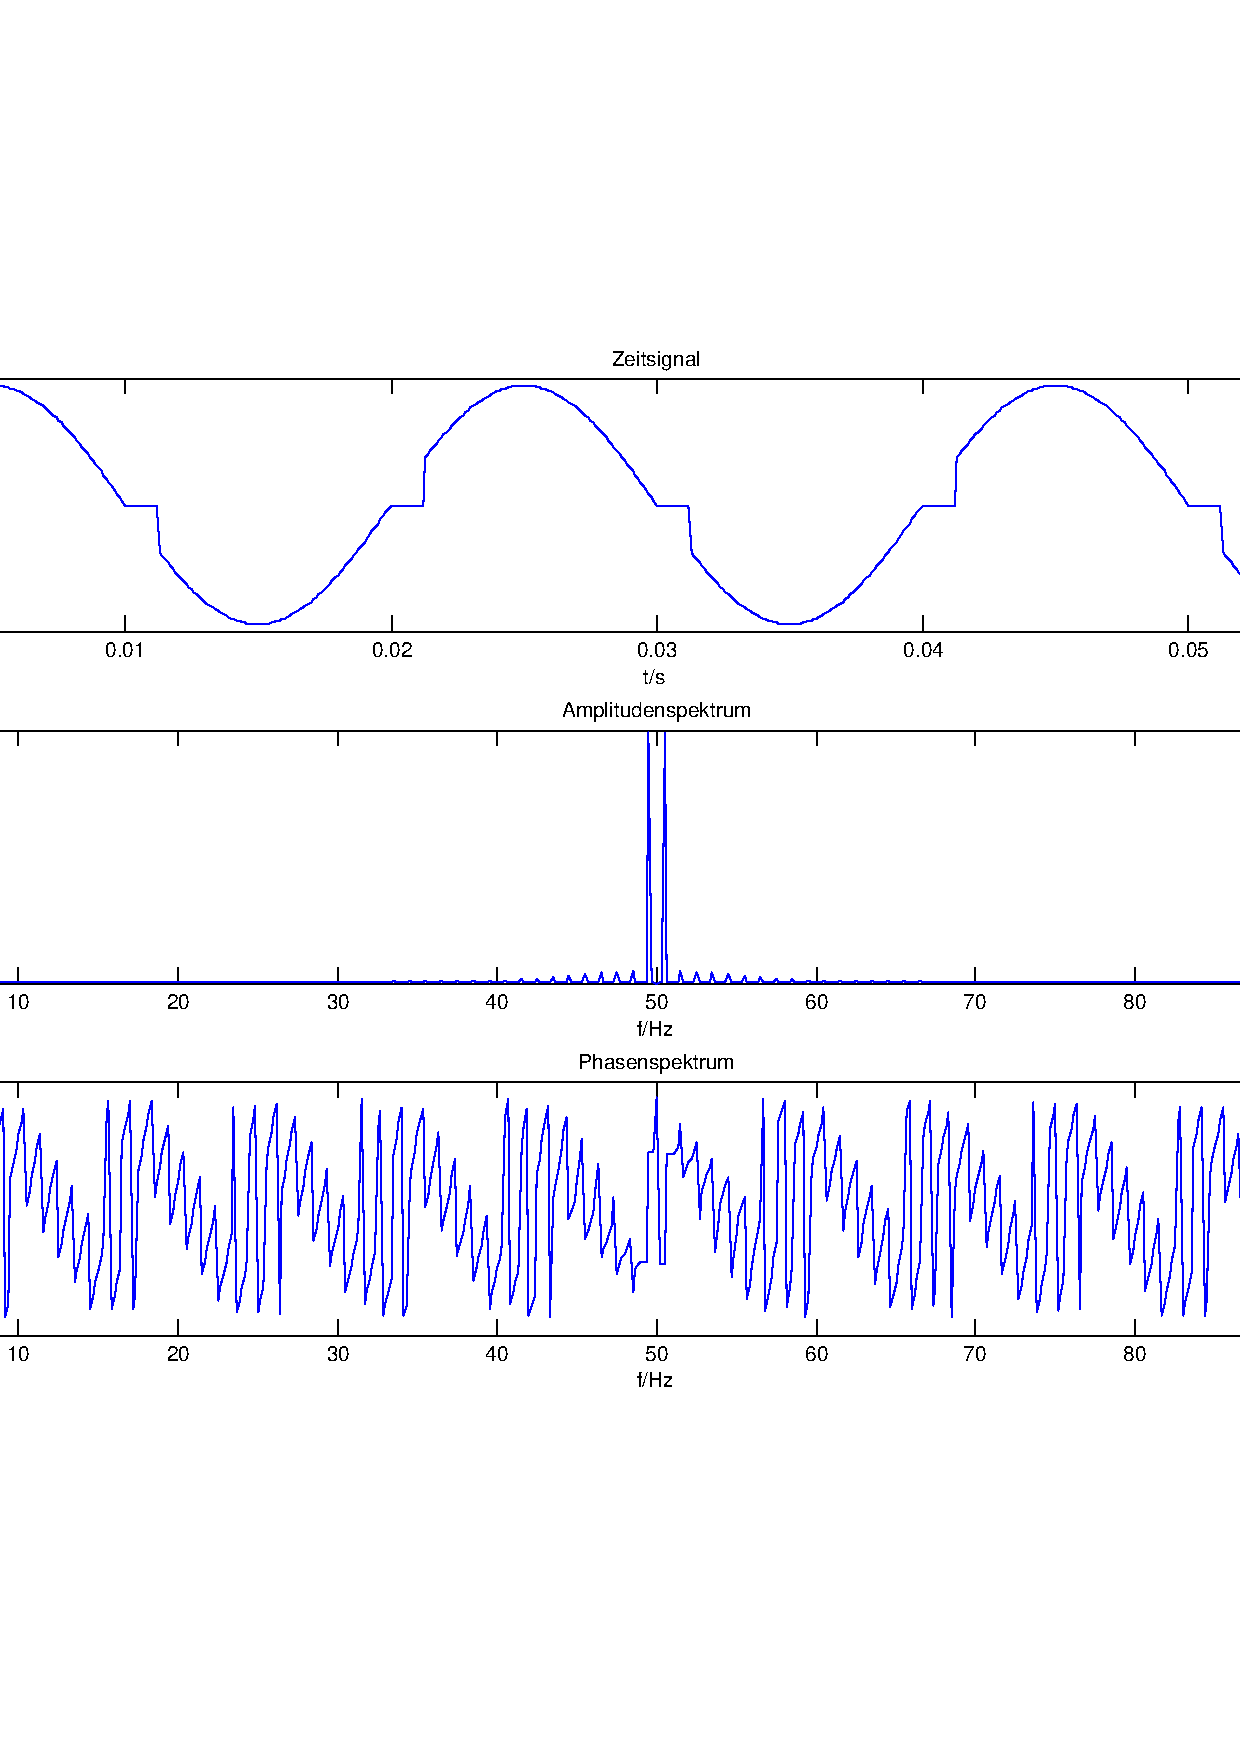
\includegraphics[scale=0.5, trim = 2cm 7cm 1.5cm 8.5cm, clip]{./Bilder/Phasenanschnitt18pi.pdf}
                        %FIXME [width=640px,
                         %height=474px]
                        \caption{Sinussignal mit Phasenanschnitt von $\frac{1}{8}/pi$}
                    \end{figure}
                \vspace{-1.5em}

                \end{minipage}

            \end{tabular}
            \end{center}

                        %4 Grafiken:
            \begin{center}
            \begin{tabular}{ll}

            \hspace{-11em}
                \begin{minipage}{0.6\textwidth}

                    \begin{figure}[H]
                        \label{fig:}
                        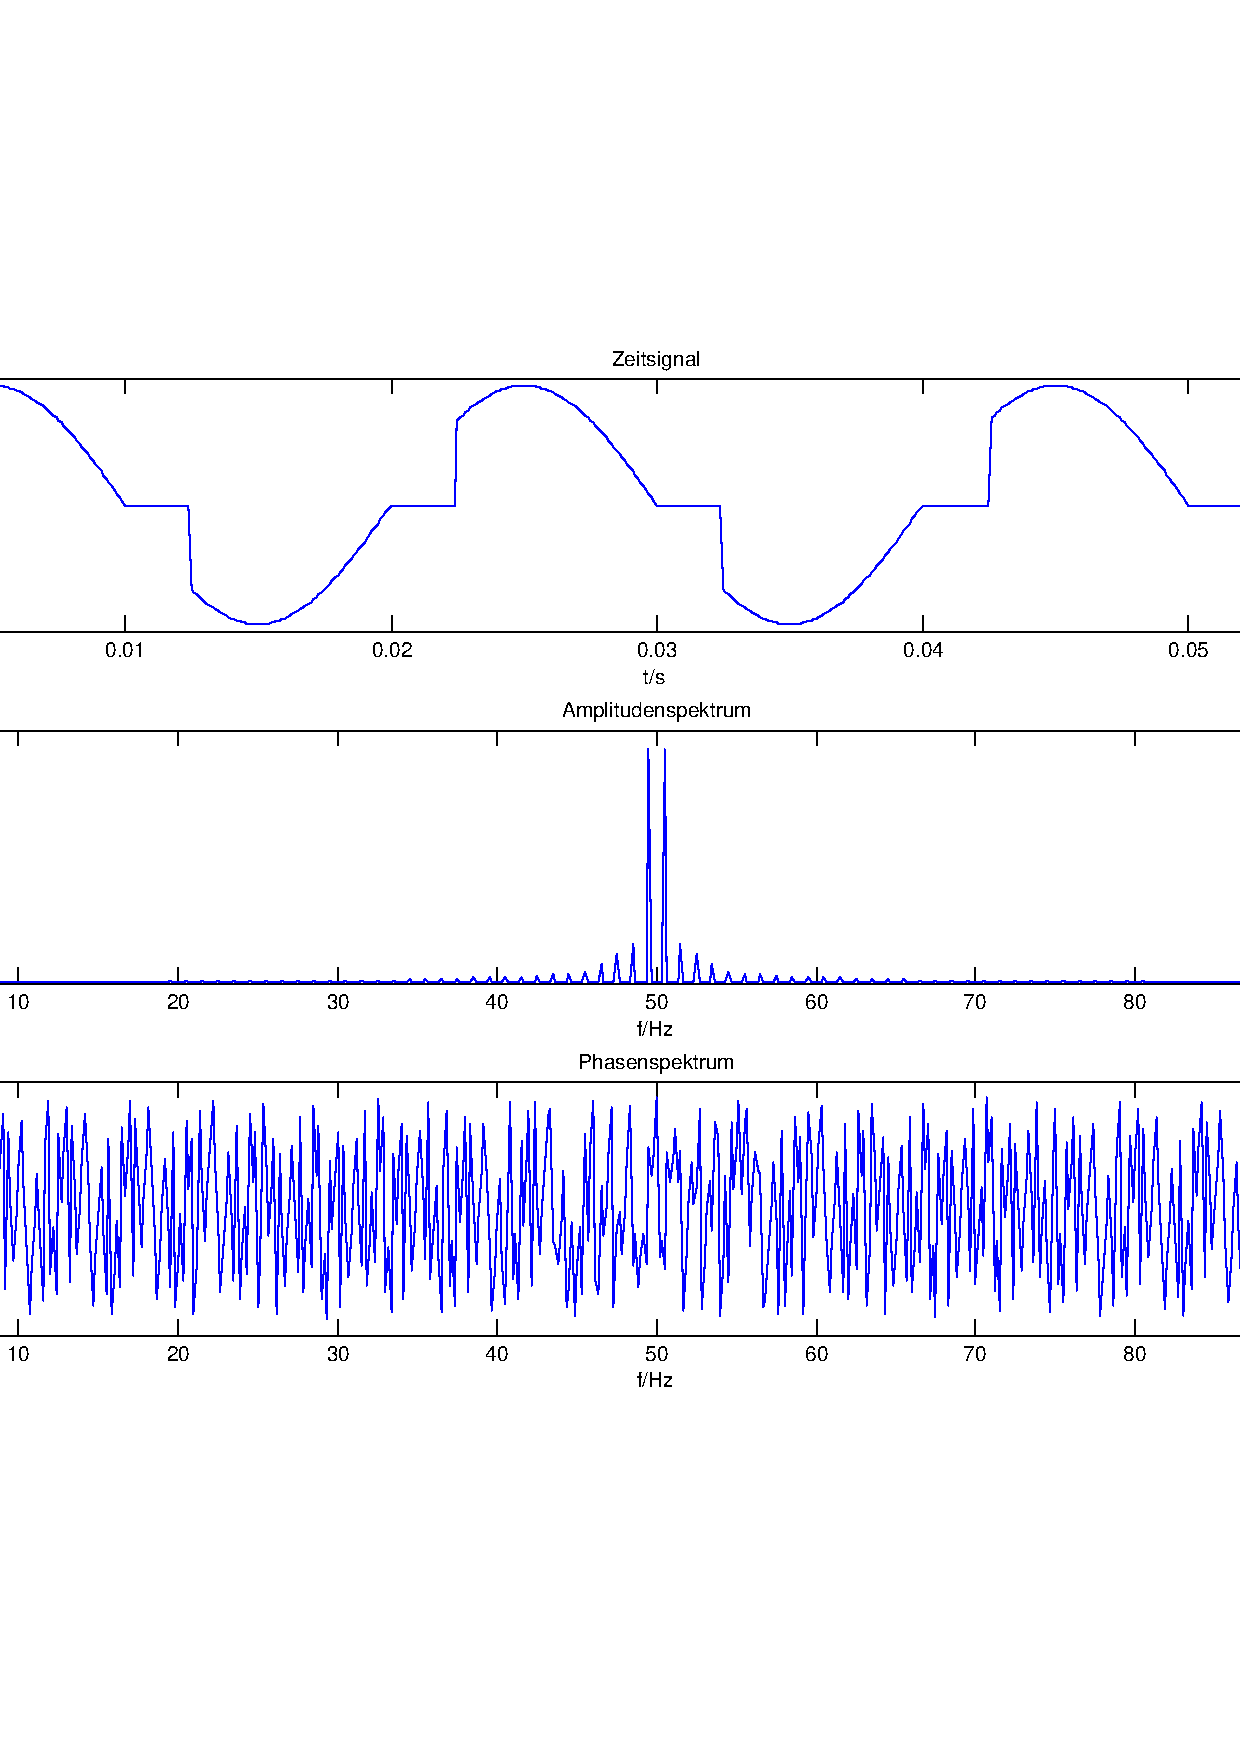
\includegraphics[scale=0.5, trim = 2cm 7cm 1.5cm 8.5cm, clip]{./Bilder/Phasenanschnitt28pi.pdf} %FIXME [width=640px,
                        % height=474px]
                        \caption{Sinussignal mit Phasenanschnitt von $\frac{1}{4}/pi$}
                    \end{figure}

                \end{minipage}
                \begin{minipage}{0.6\textwidth}

                     \begin{figure}[H]
                        \label{fig:}
                        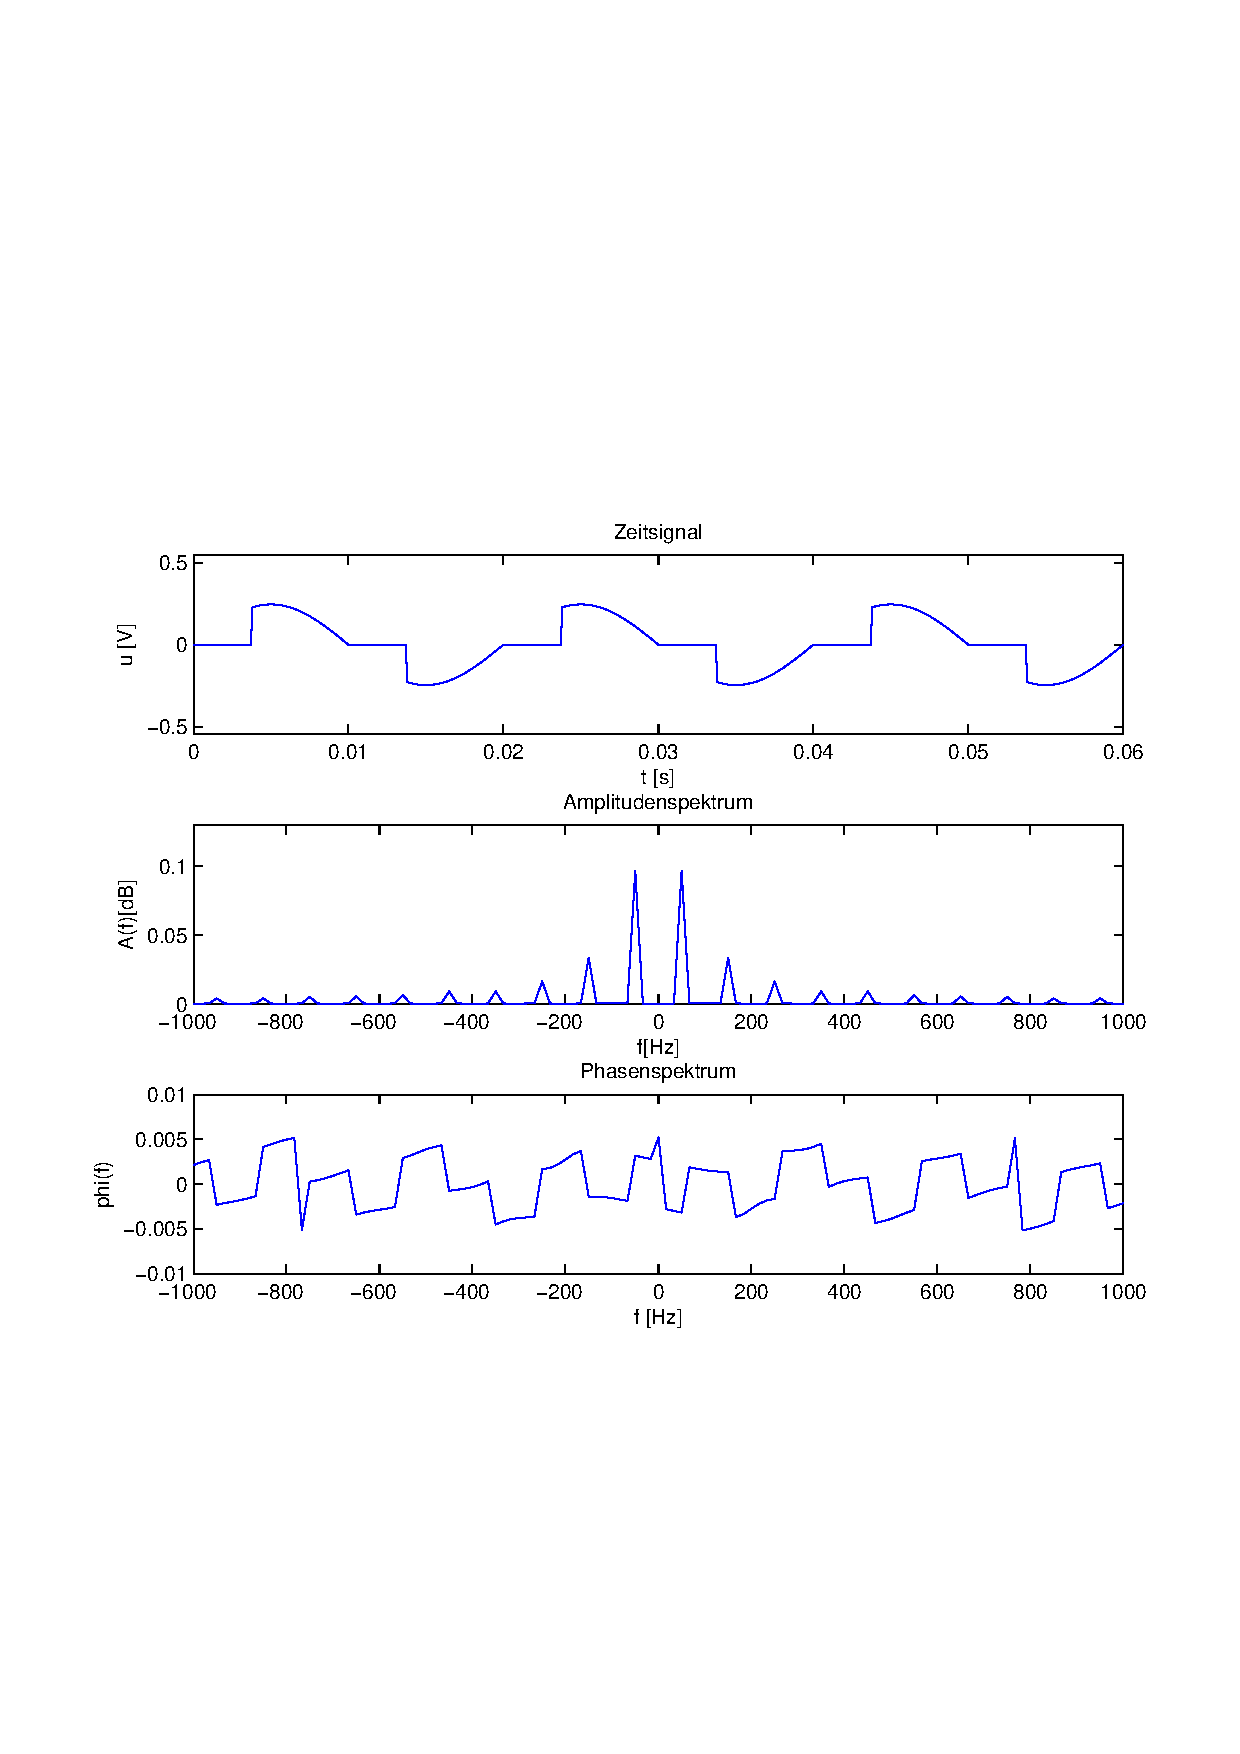
\includegraphics[scale=0.5, trim = 2cm 7cm 1.5cm 8.5cm, clip]{./Bilder/Phasenanschnitt38pi.pdf} %FIXME [width=640px,
                        % height=474px]
                        \caption{Sinussignal mit Phasenanschnitt von $\frac{3}{8}/pi$}
                    \end{figure}
               \vspace{-1.5em}

                \end{minipage}

            \end{tabular}
            \end{center}

                        %4 Grafiken:
            \begin{center}
            \begin{tabular}{ll}

            \hspace{-11em}
                \begin{minipage}{0.6\textwidth}

                    \begin{figure}[H]
                        \label{fig:}
                        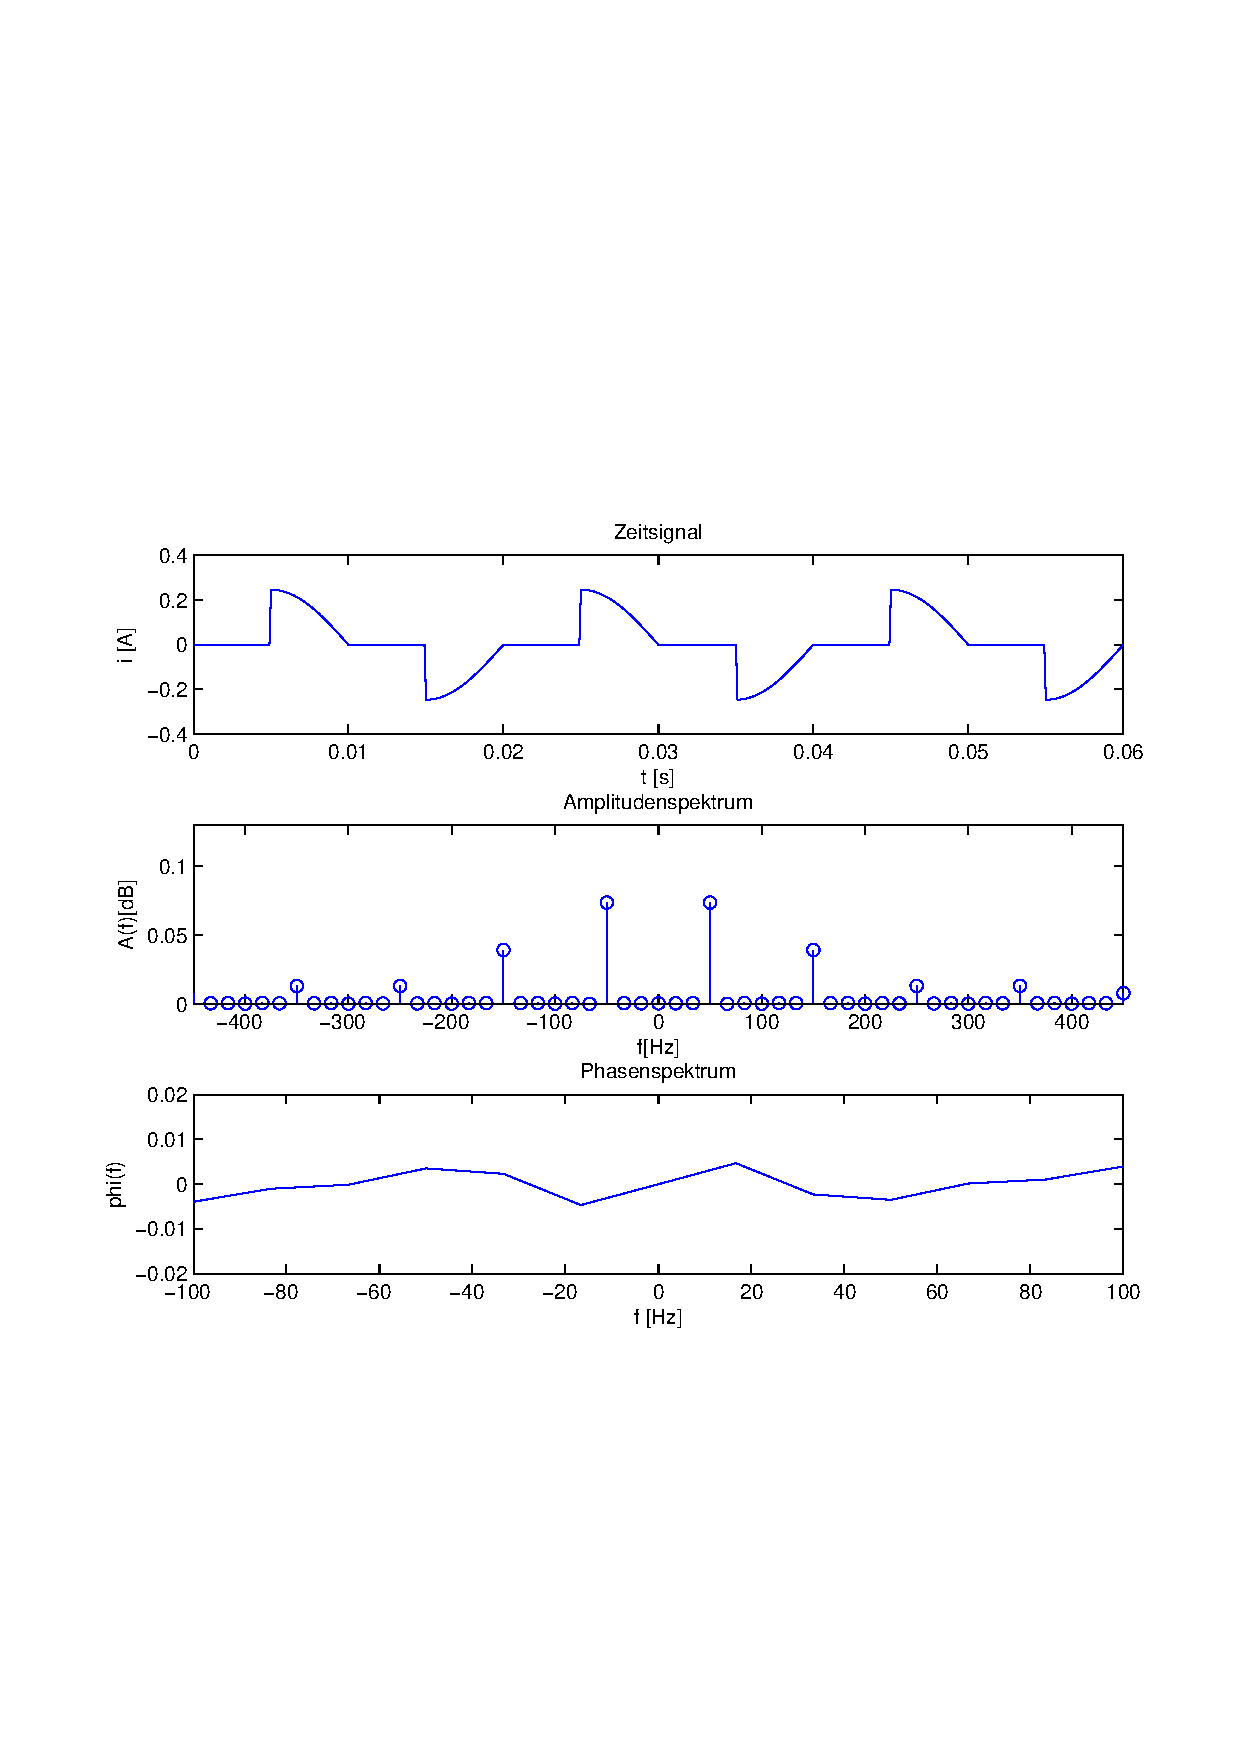
\includegraphics[scale=0.5, trim = 2cm 7cm 1.5cm 8.5cm, clip]{./Bilder/Phasenanschnitt48pi.pdf} %FIXME [width=640px,
                        % height=474px]
                        \caption{Sinussignal mit Phasenanschnitt von $\frac{1}{2}/pi$}
                    \end{figure}

                \end{minipage}
                \begin{minipage}{0.6\textwidth}

                   \begin{figure}[H]
                        \label{fig:}
                        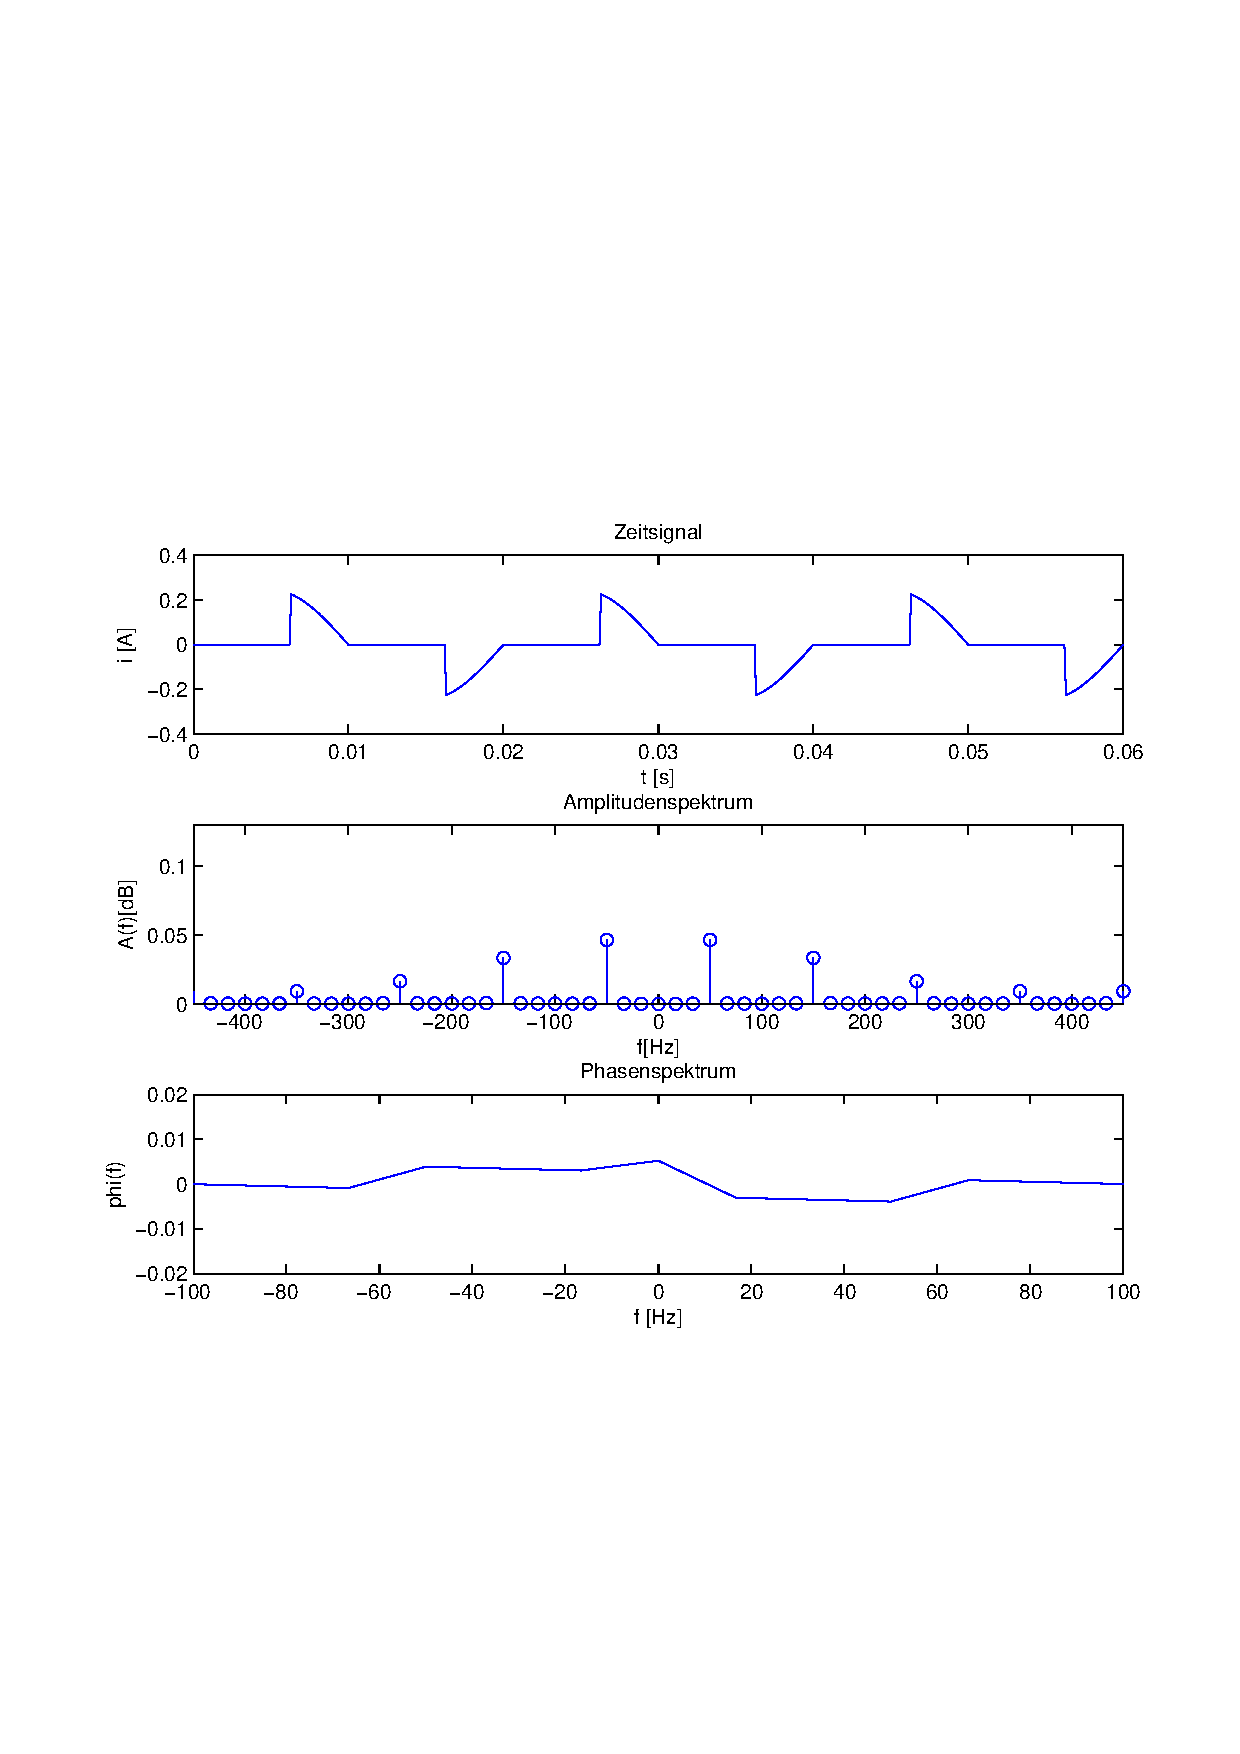
\includegraphics[scale=0.5, trim = 2cm 7cm 1.5cm 8.5cm, clip]{./Bilder/Phasenanschnitt58pi.pdf} %FIXME [width=640px,
                        % height=474px]
                        \caption{Sinussignal mit Phasenanschnitt von $\frac{5}{8}/pi$}
                    \end{figure}
                 \vspace{-1.5em}

                \end{minipage}

            \end{tabular}
            \end{center}

               %4 Grafiken:
            \begin{center}
            \begin{tabular}{ll}

            \hspace{-11em}
                \begin{minipage}{0.6\textwidth}

                    \begin{figure}[H]
                        \label{fig:}
                        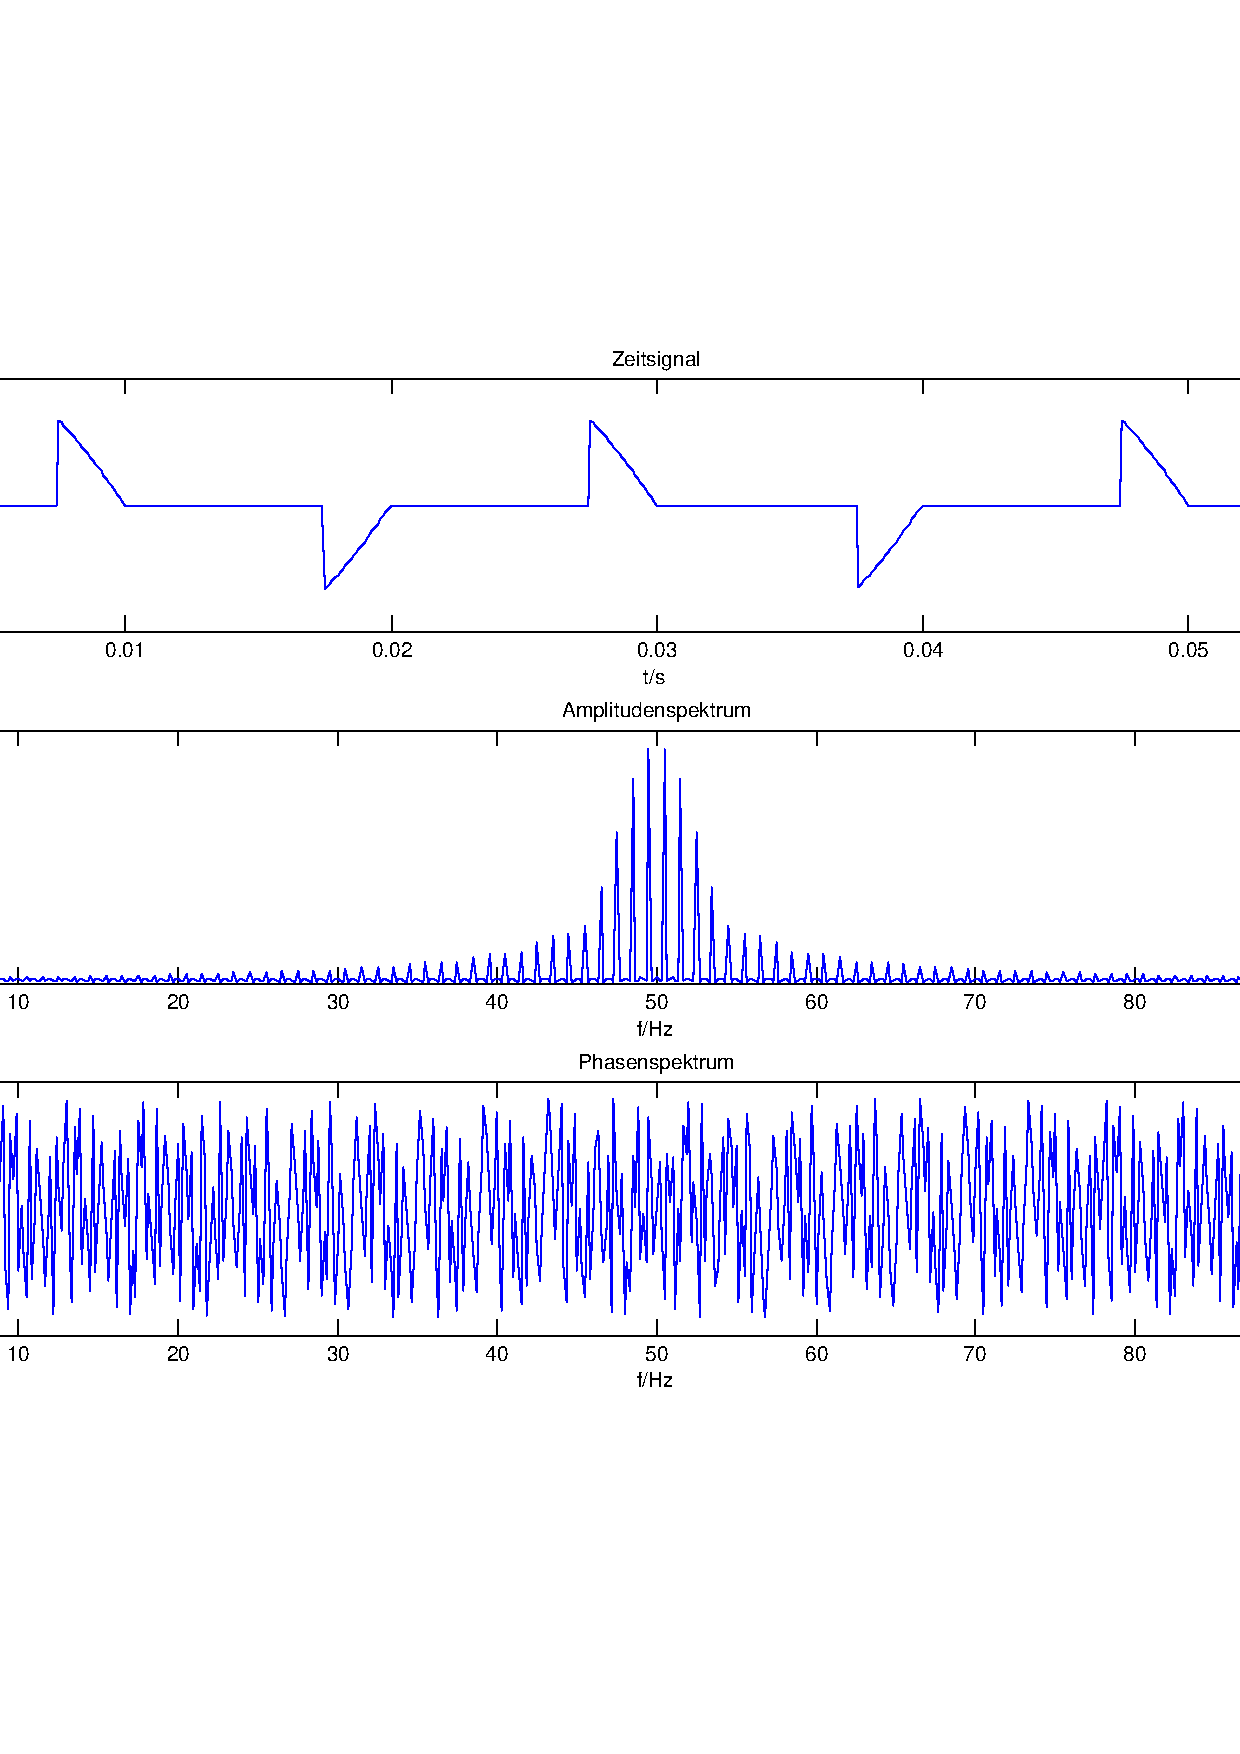
\includegraphics[scale=0.5, trim = 2cm 7cm 1.5cm 8.5cm, clip]{./Bilder/Phasenanschnitt68pi.pdf} %FIXME [width=640px,
                        % height=474px]
                        \caption{Sinussignal mit Phasenanschnitt von $\frac{3}{4}/pi$}
                    \end{figure}

                \end{minipage}
                \begin{minipage}{0.6\textwidth}

                   \begin{figure}[H]
                        \label{fig:}
                        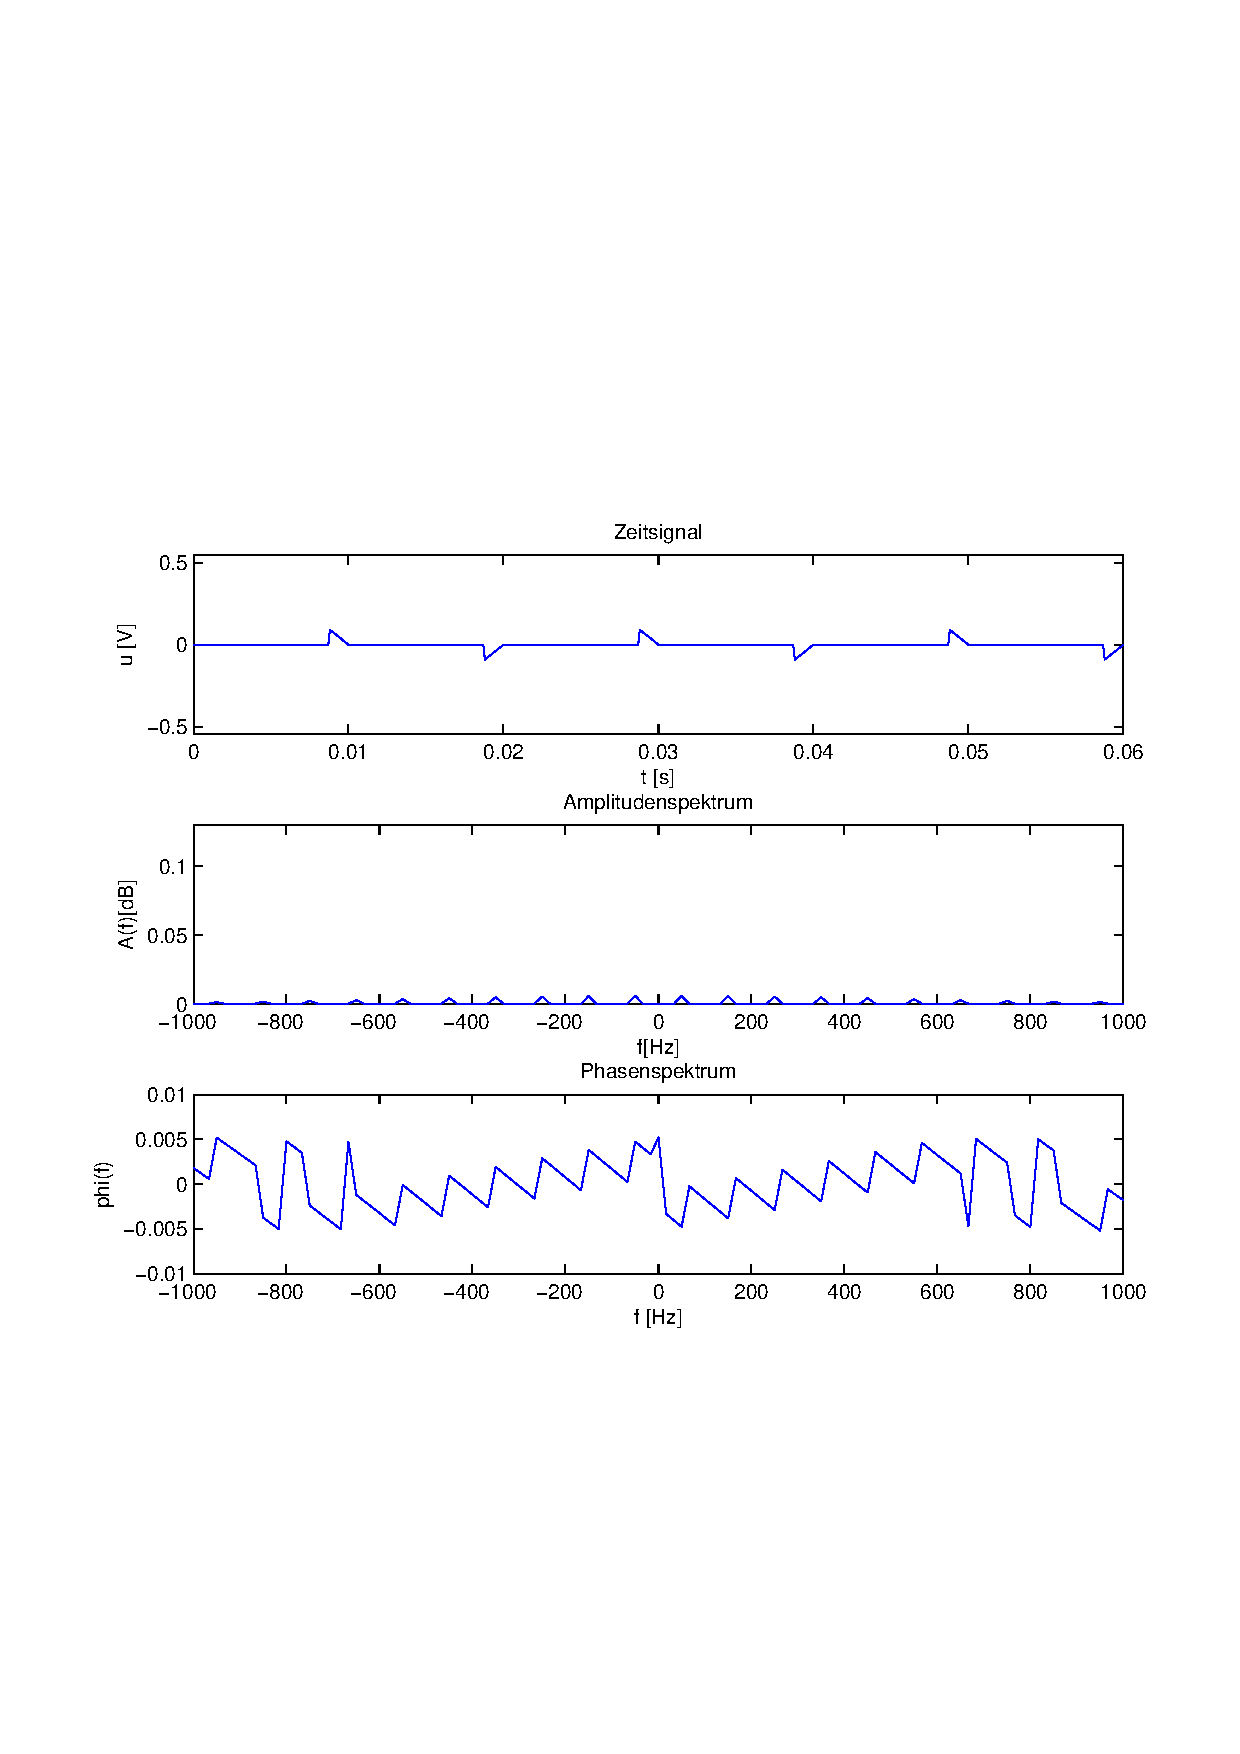
\includegraphics[scale=0.5, trim = 2cm 7cm 1.5cm 8.5cm, clip]{./Bilder/Phasenanschnitt78pi.pdf} %FIXME [width=640px,
                        % height=474px]
                        \caption{Sinussignal mit Phasenanschnitt von $\frac{7}{8}/pi$}
                    \end{figure}
                 \vspace{-1.5em}

                \end{minipage}

            \end{tabular}
            \end{center}
            
               %4 Grafiken:
            \begin{center}
            \begin{tabular}{ll}

            \hspace{-4em}
                \begin{minipage}{0.6\textwidth}

                    \begin{figure}[H]
                        \label{fig:}
                        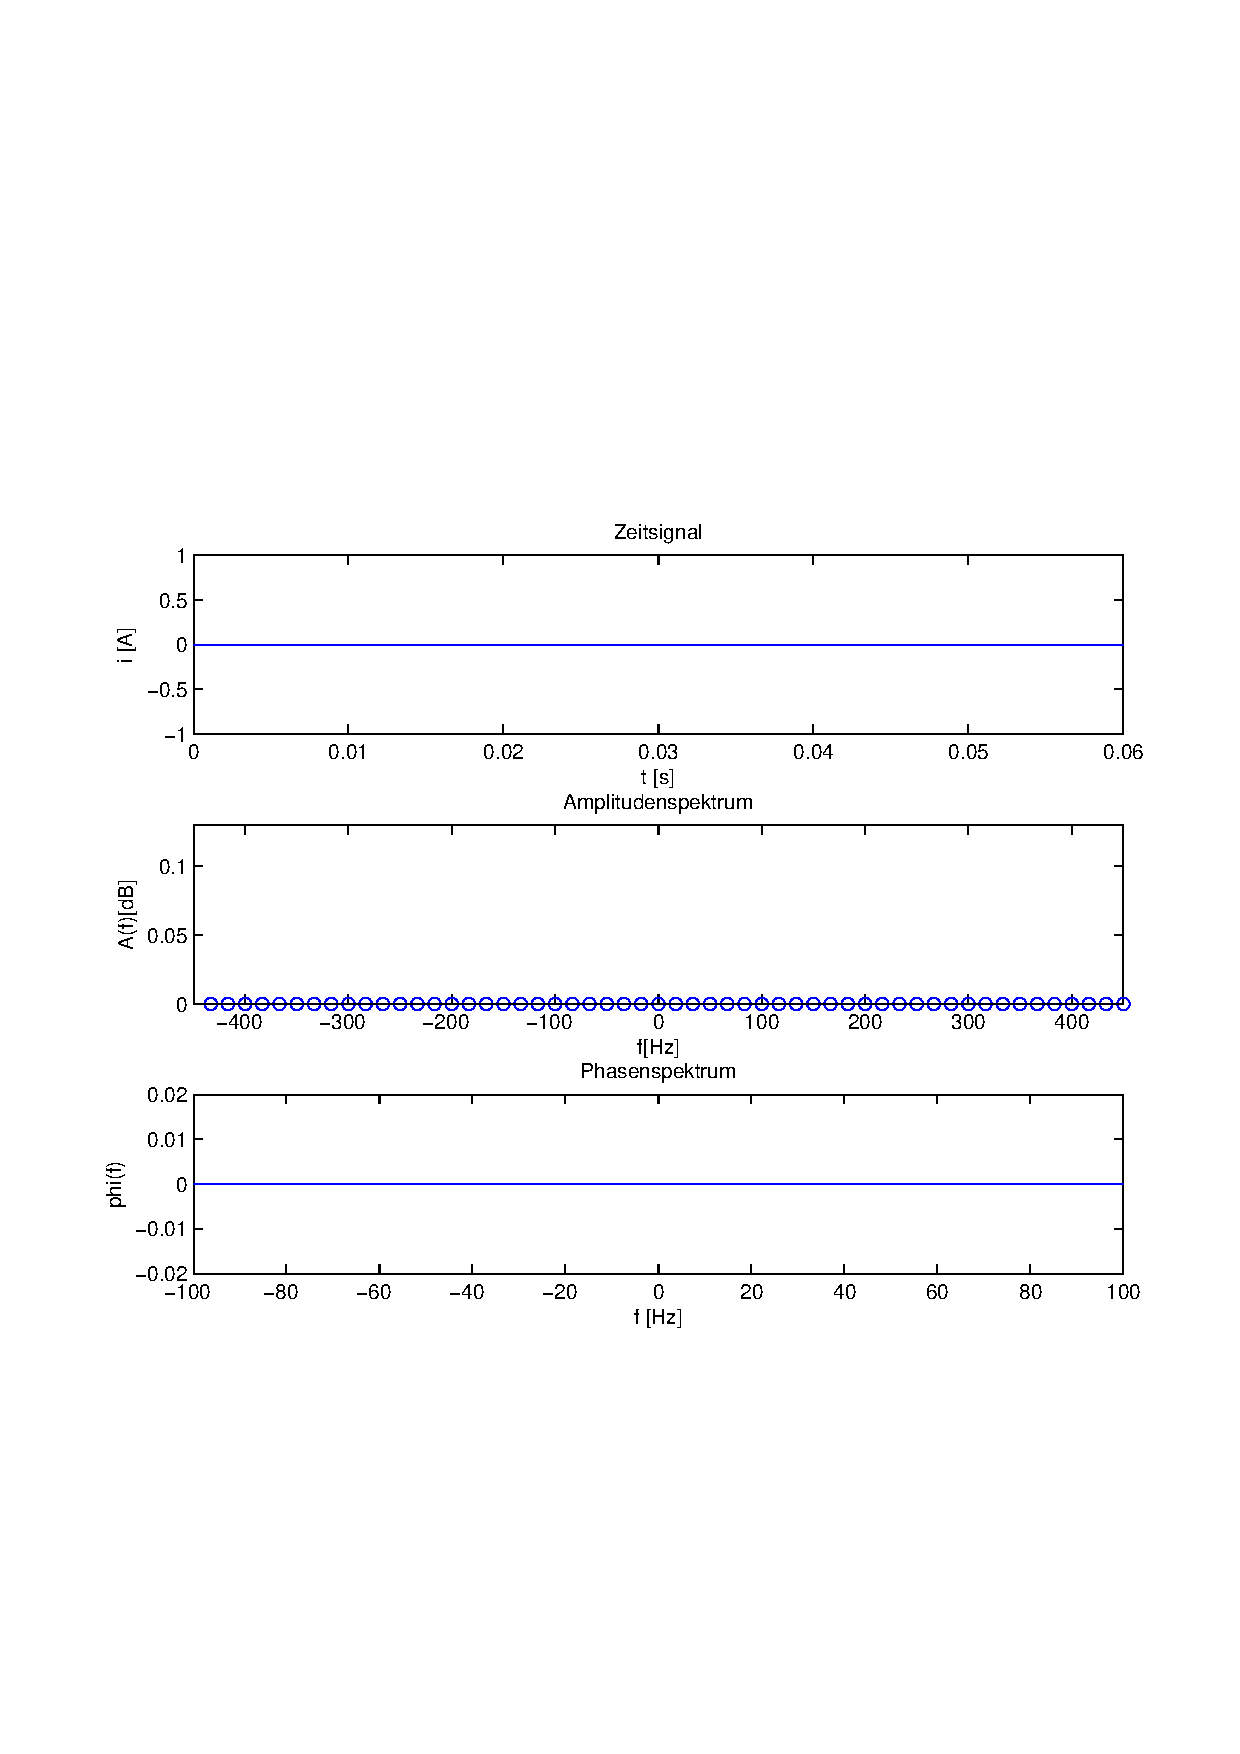
\includegraphics[scale=0.5, trim = 2cm 7cm 1.5cm 8.5cm, clip]{./Bilder/Phasenanschnitt88pi.pdf} %FIXME [width=640px,
                        % height=474px]
                        \caption{Sinussignal mit Phasenanschnitt von $/pi$}
                    \end{figure}

                \end{minipage}

            \end{tabular}
            \end{center}
             \begin{center}
                 \begin{tabular}{|c|c|c|}
                             
                   \hline
                   $\alpha $ & $i_{eff}$ (Zeitbereich) & $i_{eff}$ Frequenzbereich\\ \hline
                   $0$ & 3,5326 & 3,5326 \\ \hline
                   $\frac{1}{8} \pi$ & 3,5105 & 3,5105 \\ \hline
                   $\frac{1}{4} \pi$ & 3,3744 & 3,3744 \\ \hline
                   $\frac{3}{8} \pi$ & 3,0338 & 3,0338 \\ \hline
                   $\frac{1}{2} \pi$ & 2,5145 & 2,5145 \\ \hline
                   $\frac{5}{8} \pi$ & 1,8097 & 1,8097 \\ \hline
                   $\frac{3}{4} \pi$ & 1,0748 & 1,0748 \\ \hline
                   $\frac{7}{8} \pi$ & 0,3940 & 0,3940 \\ \hline
                   $ \pi$ & 0 & 0 \\ \hline
                         
           
                 \end{tabular}
             \end{center}        
        
        
    \end{quote}
\end{quote}

%--------------------------------------------------------------------
%--------------------------------------------------------------------

\section{Versuch}
\begin{quote}

	\subsection{Schaltungsaufbau}
	\begin{quote}
	Im praktischen Teil des Termins wurden nun reelle Messwerte aufgenommen und
	anhand der Diskreten Fouriertransformation untersucht.\\
	Dazu wurde zunächst eine Schaltung aufgebaut, in der der Strom im
	Dimmerschaltkreis erfasst werden konnte. Der Strom aus der Steckdose führt
	dabei in die Dimmerschaltung und dann in den Stromwandler der Wandler-Box. Dort
	wird das Signal in eine Spannung umgewandelt. Das Verhältnis von Strom zu
	Spannung ist bei dem Wandler linear. Bei einem Maximalstrom von $0.9 A$ kann
	man eine Maximalspannung von $\pm 10 V$ erhalten. Daher muss der Vorfaktor von
	$\frac{0.9 A}{10 V} = 0.09 \frac{A}{V}$ berücksichtigt werden. Noch in der
	Wandler-Box wird dieses Signal gefiltert und führt zum Sensorknoten, wo anhand
	der Spannungsmessung Rückschlüsse auf den Strom gemacht werden können.
	\end{quote}
	
	\subsection{MATLAB-Skript für Anschnittswinkel-Bestimmung}
	\begin{quote}	
	Als nächstes soll anhand eines selbstgeschriebenem MATLAB-Skripts der
	Anschnittswinkel der unterschiedlichen Signale bestimmt werden. Die
	Anschnittswinkel werden dafür vorher mit dem Oszilloskop eingestellt. Da es
	manuell nicht so einfach ist, wurden kleine Abweichungen toleriert. Hier eine
	Tabelle der Anschnittswinkel mit den dazugehörigen Zeitlängen, in denen das
	Signal nicht in der normale Sinusperiode verläuft:
	
	   \begin{center}
                 \begin{tabular}{|c|c|c|}
                             
                   \hline
                   Anschnittswinkel & $t\ [ms]$ erwünscht & $t\ [ms]$
                   eingestellt\\ \hline 
                   $\frac{1}{8} \pi$ & 1.25 & 1.2 \\ \hline
                   $\frac{1}{4} \pi$ & 2.5 & 2.4 \\ \hline
                   $\frac{3}{8} \pi$ & 3.75 & 3.6 \\ \hline
                   $\frac{1}{2} \pi$ & 5 & 5 \\ \hline
                   $\frac{5}{8} \pi$ & 6.25 & 6.2 \\ \hline
                   $\frac{3}{4} \pi$ & 7.5 & 7.6 \\ \hline
                   $\frac{7}{8} \pi$ & 8.75 & 8.6 \\ \hline                         
           
                 \end{tabular}
       \end{center}        
       
    Das dazugehörige Skript ist am Ende des Protokolls zu sehen.\\
    
    Im Vergleich zwischen den am Oszilloskop abgelesenen Werten und den MATLAB
    Ergebnissen können wir sehen, dass wir entweder echt hammermäßige oder toal
    bekloppte Ergebnisse haben!!
	\end{quote}
	
	\subsection{Amplituden- und Phasenspektrum des Stroms anhand der Diskreten
	Fouriertransformation}
	\begin{quote}
	\end{quote}
	
	\subsection{Effektivwert des Stroms im Zeit- und Frequenzbereich}
	\begin{quote}
	Zuletzt sollte der Effektivwert des Stroms einer Messung im Zeit- und
	Frequenzbereich ermittelt werden, indem der MATLAB-Skript der
	Vorbereitungsaufgabe verwendet wurde. Wir verwendeten den Strom des Signals bei
	einem Anschnittswinkel von $\frac{\pi}{2}$.\\
	Das MATLAB-Skript gibt uns das Ergebnis von $0.21 A$ für Zeit- und
	Frequenzbereich. Der mithilfe des Multimeters gemessene Strom beträgt $0.224
	A$.\\
	
	Vergleicht man beide Messungen, kann man sehen, dass es keine erhebliche
	Differenz gibt.
	
	 
	\end{quote}
\end{quote}

%--------------------------------------------------------------------
%--------------------------------------------------------------------

\section{Ergebnisse}
\begin{quote}
	
\end{quote}

%--------------------------------------------------------------------
%--------------------------------------------------------------------
\section{Quellcode}
\begin{quote}
    \subsection{sinus2.m}
    \begin{quote}
        \lstinputlisting[
            caption={sinus2},
            label=lst:Matlab]
            {./Matlab/sinus2.m}
    \end{quote}
    \subsection{stromPhasSchnitt.m}
    \begin{quote}
        \lstinputlisting[
            caption={stromPhasSchnitt},
            label=lst:Matlab]
            {./Matlab/stromPhasSchnitt.m}
    \end{quote}
    \subsection{EffektivwertZeitbereich.m}
    \begin{quote}
        \lstinputlisting[
            caption={EffektivwertZeitbereich},
            label=lst:Matlab]
            {./Matlab/EffektivwertZeitbereich.m}
    \end{quote}
    \subsection{EffektivwertFourier.m}
    \begin{quote}
        \lstinputlisting[
            caption={EffektivwertFourier},
            label=lst:Matlab]
            {./Matlab/EffektivwertFourier.m}
    \end{quote}
	
\end{quote}

%--------------------------------------------------------------------
%--------------------------------------------------------------------


\begin{thebibliography}{999}
%\bibitem {DigitaleMesskette} Prof. Dr.-Ing. Gühmann, Clemens: MDVScript\_01, S.5

%Name, Vorname.; evtl. Name2, Vorname2.: Titel des Dokumentes
%oder Buches, Zeitschrift/Verlag/URL (Auflage, Erscheinungsort, -jahr), ggf. Seitenzahlen
%\bibitem [Wiki10] {DigitaleMesskette2} \url{www.wikipedia.org}, Zugriff 22.03.2010
\end{thebibliography}


\end{document}


